\chapter{Plataforma de desarrollo}
\label{cap:capitulo4}

\vspace{1cm}

En este capítulo se describen las plataformas de desarrollo utilizadas para la implementación del dispositivo propuesto. En concreto, se detallan los componentes hardware empleados en la construcción del pastillero automatizado, así como las herramientas software utilizadas para su programación, diseño e interacción con el usuario. Todo ello se ha seleccionado siguiendo una filosofía de bajo coste, garantizando al mismo tiempo el correcto funcionamiento del sistema en tiempo real.\\

\section{Hardware}

En este apartado se describen los componentes hardware utilizados en el desarrollo del sistema. La selección de los elementos se ha realizado buscando siempre el bajo coste del dispositivo, priorizando componentes accesibles, fáciles de integrar y adecuados para un funcionamiento en tiempo real.\\

El sistema se compone de un microcontrolador principal encargado del procesamiento y control, una interfaz de usuario basada en pantalla táctil resistiva, un sensor biomédico para la monitorización del pulso y la saturación de oxígeno en sangre (SpO2), así como la estructura física del pastillero diseñada mediante impresión 3D. Además, se incluyen los elementos necesarios para la comunicación inalámbrica y la alimentación del dispositivo.

\subsection{Microcontrolador ESP32-2432S028}

El núcleo del sistema está compuesto por un microcontrolador conocido como ESP32-2432S028, el cual se basa en el chip ESP32 y combina, dentro de un solo módulo, la capacidad de procesamiento, la comunicación inalámbrica y el control de periféricos.\\

Este microcontrolador destaca por incorporar conectividad WiFi y Bluetooth de forma nativa, lo que facilita la comunicación directa con la aplicación móvil sin requerir módulos adicionales. De este modo, disminuyen tanto el costo como la complejidad del sistema. Además, cómo se muestra en la Figura \ref{fig:esp32}, tiene suficientes pines GPIO (de entrada/salida) para conectar sensores, actuadores y la pantalla táctil que viene incorporada.\\

\begin{figure}[H]
    \centering
    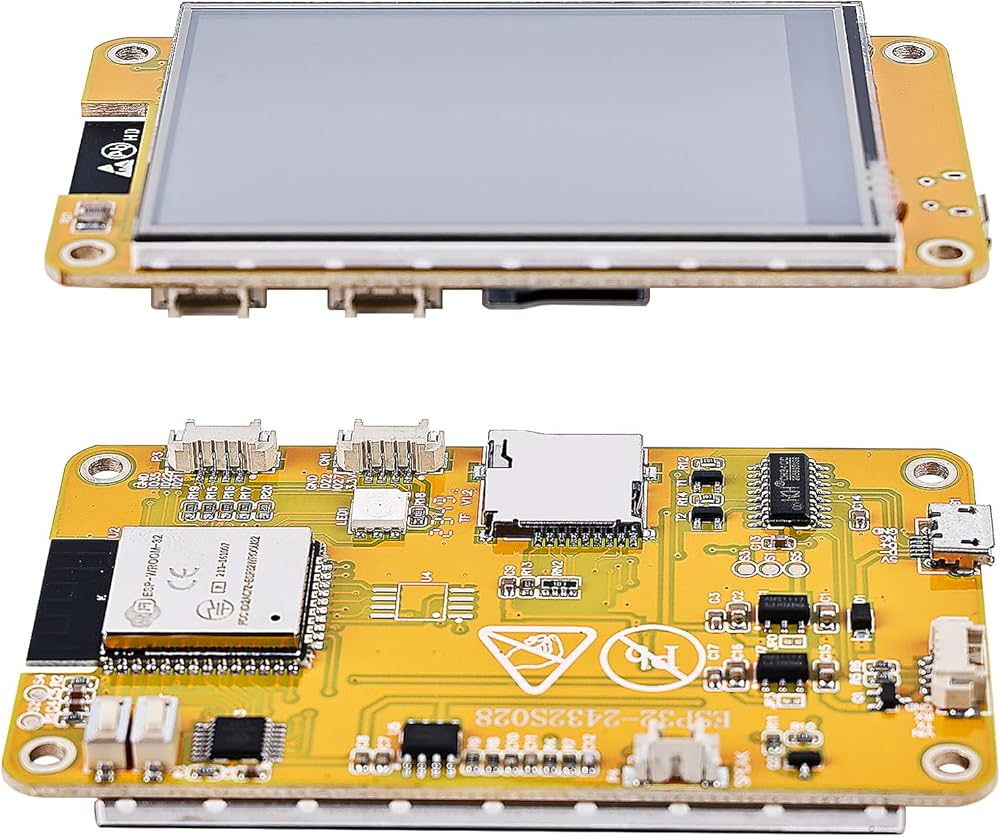
\includegraphics[width=0.6\textwidth]{figs/esp32.jpg}
    \caption{Microcontrolador ESP32-2432S028 utilizado en el sistema.}
    \label{fig:esp32}
\end{figure}

Una de las principales vetajas de este modelo es que incluye una pantalla TFT de 2.8 pulgadas con interfaz táctil resistiva, lo cual posibilita la integración de una interfaz para el usuario directamente en el dispositivo. Esto es importante para el proyecto ya que permite interactuar con el usuario sin tener que depender únicamente de la aplicación móvil.\\

En cuanto a su capacidad de procesamiento, el ESP32 cuenta con un procesador de doble núcleo que permite gestionar múltiples tareas de forma eficiente, como la lectura de sensores, la actualización de la interfaz gráfica.

\subsubsection{Pantalla táctil}

La pantalla táctil resistiva que viene integrada en el microcontrolador constituye el principal medio de interacción directa entre el usuario y el dispositivo. El uso de una pantalla táctil permite mostrar información relevante de forma clara e intuitiva, como recordatorios de medicación, estados del sistema o lecturas del sensor biomédico. Asimismo, posibilita la interacción directa mediante pulsaciones, evitando la necesidad de botones físicos adicionales y simplificando el diseño del dispositivo.\\

Además, una interfaz táctil resistiva es más económica frente a otro tipo de tecnologías como podría ser la capacitiva, lo que beneficia a que el dispositivo sea de bajo coste y más resistente en entornos domésticos. Por otro lado, teniendo en cuenta el perfil del usuario que emplearía este sistema, las pantallas táctiles resistivas presentan la ventaja de poder ser usadas con cualquier objeto o incluso con guantes.\\

Desde el punto de vista del diseño de la interfaz, se ha priorizado la simplicidad y la claridad visual, empleando elementos gráficos de gran tamaño y fácil identificación. Esto facilita el uso del dispositivo por parte de personas mayores o con poca experiencia en el uso de tecnologías digitales.\\

En conjunto, la pantalla táctil no solo actúa como elemento de visualización, sino que constituye un componente fundamental para mejorar la accesibilidad y la usabilidad del sistema.

\subsection{Sensor de pulso y SpO2}

Para monitorizar los parámetros biomédicos del usuario, se ha utilizado un sensor MAX30102. Este sensor permite medir de forma no invasiva tanto la frecuencia cardíaca como el nivel de oxigenación en sangre, siendo ampliamente utilizado en dispositivos portátiles de salud.\\

\begin{figure}[H]
    \centering
    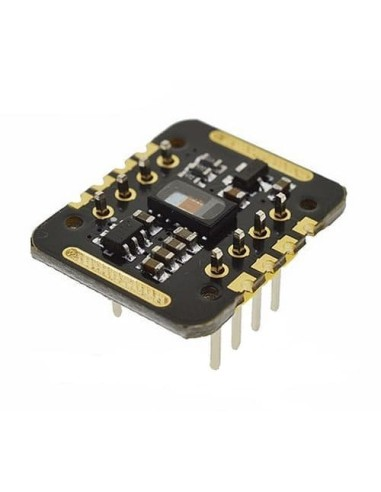
\includegraphics[width=0.35\textwidth]{figs/max30102.jpg}
    \caption{Sensor MAX30102 utilizado para la medición de pulso y SpO2.}
    \label{fig:max30102}
\end{figure}

El funcionamiento del sensor se basa en emitir luz a través de la piel, normalmente en longitudes de onda roja e infrarroja, midiendo la variación de la luz absorbida por la sangre. A partir de estas mediciones, es posible estimar tanto el pulso como la saturación de oxígeno.\\

Como se puede observar en la Figura \ref{fig:max30102}, el sensor presenta un tamaño reducido y una fácil integración con sistemas embebidos, lo que lo hace especialmente adecuado para aplicaciones portátiles y de bajo consumo.\\

La comunicación con el microcontrolador se realiza mediante el protocolo I2C, lo que permite una conexión sencilla utilizando un número reducido de pines. La incorporación de este sensor en el sistema permite añadir una funcionalidad adicional de seguimiento de la salud del usuario, complementando el objetivo principal del pastillero automatizado y aportando un mayor valor al dispositivo.

\subsection{Diseño mecánico del sistema}

El diseño mecánico del sistema se ha centrado en el desarrollo de un pastillero automatizado que permita almacenar y dispensar medicamentos de forma organizada, accesible y segura en un entorno doméstico. Para ello, se ha diseñado una estructura compacta que integra los distintos componentes del sistema, como el microcontrolador, el sensor biomédico y la interfaz de usuario.\\

El modelado del dispositivo se ha realizado en 3D, lo que ha permitido definir con precisión la disposición de los componentes y realizar iteraciones del diseño hasta alcanzar una solución funcional y ergonómica. Se ha priorizado la facilidad de uso, empleando una disposición que facilite tanto la interacción con la pantalla como el acceso a los compartimentos de medicación.\\

La fabricación de las piezas se ha llevado a cabo mediante impresión 3D utilizando filamento PLA, seleccionado por su bajo coste y facilidad de uso en prototipado. Para ello, se han empleado dos impresoras distintas: una Creality Ender 3 y una Bambu Lab P1S Combo. El uso de ambas ha permitido observar diferencias en la calidad de impresión, especialmente en la precisión dimensional y el acabado superficial, lo que influye en el ajuste entre piezas y en el resultado final del dispositivo.\\

Finalmente, el diseño se ha planteado de forma modular, permitiendo futuras modificaciones o ampliaciones del sistema sin necesidad de rediseñar completamente la estructura.

